\section{Experiments}
\label{sec:experiments}

We test the population predictions on a language model trained with the actual IPO and DPO losses. The test is quantitative. For every run, the exact recursion of \Cref{sec:hodge}, evaluated on the same panels, preference oracle, and hyperparameters, fixes in advance the trajectory and the target that the trained model should reach, and the hypotheses with their pass criteria were frozen before training.

\subsection{Setup}
\paragraph{Panels.} The policy is Qwen2.5-0.5B-Instruct, fully fine-tuned. Prompts are open-ended requests that admit several short answers: 65 templated requests for names, slogans, titles, recommendations, and descriptions, and the NoveltyBench prompts~\citep{zhang2025noveltybench}, each with the instruction to answer in at most six words. For each prompt the initial model draws 48 answers, and the four most probable distinct complete answers form a fixed panel. A panel is kept when every answer has initial panel probability at least $0.05$, so that the initial policy is interior; 130 of 600 prompts qualify.

\paragraph{Feedback.} Every answer is scored by the Bradley--Terry reward model Skywork-Reward-Llama-3.1-8B-v0.2. Soft labels $P^*_{ij}=\sigma((r_i-r_j)/T)$ with $T=3.17$ are Bradley--Terry, hence additive under the logit link; hard labels $P^*_{ij}=\mathbf 1[r_i>r_j]$ are what a scalar oracle that compares scores produces. Cycles are studied with a labelled planted-cycle oracle on the same panels (\Cref{sec:exp-cycles}).

\paragraph{One round.} With $s_t(i)$ the sequence log-probability of panel answer $i$ under the current model, the round uses the reference scores $\alpha s_t+(1-\alpha)s_0$, the sampler $\bmu_t=(1-\lambda)\,\mathrm{unif}+\lambda\,\softmax(s_t)$, and the pairwise loss $\sum_{i\neq j}\mu_{t,i}\mu_{t,j}\,\ell(h_i-h_j)$ in the log-ratios $h=s_\theta-(\alpha s_t+(1-\alpha)s_0)$, where $\ell$ is the IPO square loss $(h_i-h_j-\beta(P^*_{ij}-\tfrac12))^2$ or the DPO logistic loss with soft labels and coefficient $1/\beta$. At its optimum this round is exactly MRS-$\Psi$PO, with the identity link for IPO and, for Bradley--Terry labels, the logit link for DPO. We take 40 Adam steps per round from a fresh optimizer; across the runs, the median per-round deviation of the trained panel scores from the exact round map, applied to the model's own state, is 0.092 nats. All population curves below start from the same initial scores as the run they are compared with.

\subsection{Target sharpness decides where the loop goes}
\label{sec:exp-sharpness}
\Cref{prop:target} predicts that configurations with the same $B=\beta/(1-\alpha)$ share their target. Four IPO runs with $B=8$, from a fixed reference with $\beta=8$ to slow refresh with $\alpha=0.9$ and $\beta=0.8$, end at the same panel policy: the largest pairwise KL between their final policies is 0.0076 nats, and their KL to the population target ranges from 0.0008 to 0.0067 nats, while the control with $B=2$ ends at KL 0.207--0.227 from them (\Cref{fig:exp-sharpness}(a)). The refresh weight changes only the approach, at the rate $\alpha$. With $\beta=1$ fixed, raising $\alpha$ raises the sharpness, and the entropy of each run levels off at the population target for $B=1/(1-\alpha)$; plotted against $M_t(\alpha)$, the curves of different $\alpha$ coincide until each saturates (\Cref{fig:exp-sharpness}(b)). Final entropies: $\alpha=0.5$: 1.085 (target 1.087); $\alpha=0.8$: 0.940 (target 0.943); $\alpha=0.9$: 0.691 (target 0.689); $\alpha=0.95$: 0.415 (target 0.410).

\begin{figure}[t]
\centering
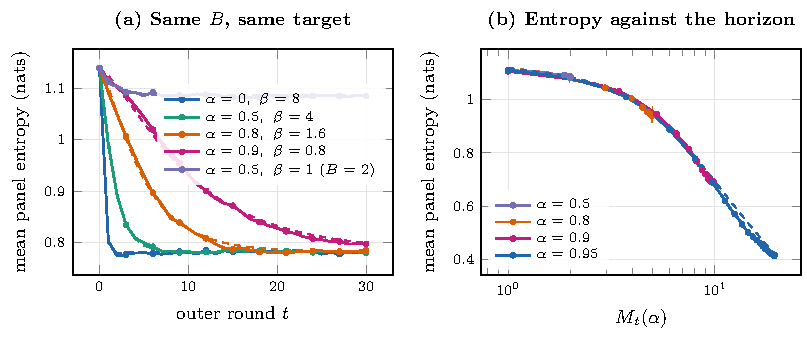
\includegraphics[width=0.98\textwidth]{exp_sharpness.pdf}
\caption{Target sharpness in neural IPO (solid, with markers) against the exact population recursion (dashed). \textbf{(a)} Four configurations with $B=\beta/(1-\alpha)=8$ reach the same panel entropy and policy; the control with $B=2$ does not. \textbf{(b)} At $\beta=1$, entropy against the horizon $M_t(\alpha)$ follows one curve until each run saturates at its own target.}
\label{fig:exp-sharpness}
\end{figure}

\subsection{The link decides whether there is a finite target}
\label{sec:exp-link}
At $\alpha=0.8$ and $\beta=1$ (\Cref{fig:exp-link}(a)), DPO with soft Bradley--Terry labels levels off at entropy 0.388 against the predicted 0.385 (KL to the target 0.0005), and IPO with hard labels levels off at 0.677 against 0.679. DPO with the same hard labels has no finite target: its panel entropy is 0.007 after one round, and the log-odds between its two most probable answers keep growing at every later round despite the anchor, as the deterministic-label analysis of \Cref{sec:concentration} predicts.

\subsection{Full refresh concentrates on the Condorcet winner}
Under full refresh with hard labels and on-policy sampling, the hard order has a Condorcet winner on every panel, and \Cref{cor:sst} predicts concentration on it. The trained model puts its largest mass on the Condorcet winner on 100\% of the panels after the last round, with mass at least $0.95$ on 100\% of them, tracking the population curve (\Cref{fig:exp-link}(b)).

\begin{figure}[t]
\centering
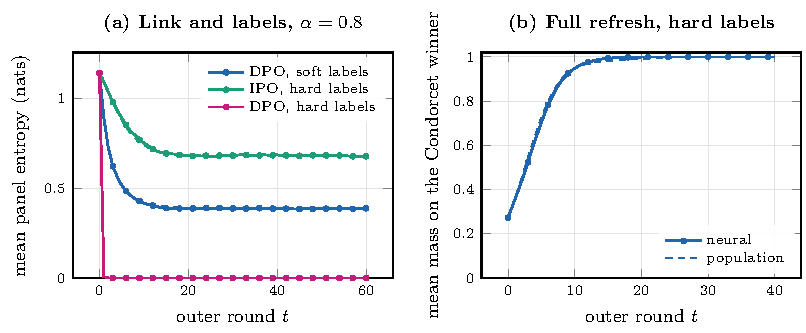
\includegraphics[width=0.98\textwidth]{exp_link_fullrefresh.pdf}
\caption{\textbf{(a)} Link and labels at $\alpha=0.8$: soft-label DPO and hard-label IPO level off at their population targets (dashed), while hard-label DPO collapses in the first round. \textbf{(b)} Full refresh with hard labels: mean mass on the Condorcet winner, neural against population.}
\label{fig:exp-link}
\end{figure}

\subsection{Cycles: nonconvergence where the theory predicts it}
\label{sec:exp-cycles}
Natural feedback rarely produces candidate sets without a Condorcet winner (\Cref{sec:exp-practice}), so we plant one, on 64 of the panels. On each panel three answers form a rock--paper--scissors cycle of strength $q=0.3$ and the fourth loses to all; half the panels are balanced ($\Delta=0.05<q/2$, a majority cycle whose maximal lottery has three answers) and half decisive ($\Delta=0.2$, a Condorcet winner). The population model predicts, before training, which configurations hold their target. At fixed $\beta=4$, balanced panels are stable at $\alpha=0.5$ and unstable at $\alpha=0.9$ and $0.95$; at the fixed target $B=12$, they are unstable at $\alpha=0.2$ and $0.5$ and stable at $\alpha=0.8$ and $0.9$; decisive panels concentrate and stay stable throughout. We call a panel oscillating when, over the last 30 of 80 rounds and after removing a linear trend, the probability of some answer still varies with standard deviation above four times the noise floor of the converged runs of \Cref{sec:exp-sharpness}; we measure on probabilities rather than logits because the pairwise loss places almost no weight on answers of vanishing probability, whose logits then wander without affecting the policy. \Cref{fig:exp-cycles}(a) compares, configuration by configuration, the share of oscillating panels with its prediction: for balanced panels it is 0\% (predicted 0\%), 100\% (predicted 100\%), 100\% (predicted 100\%), 100\% (predicted 100\%), 94\% (predicted 91\%), 0\% (predicted 0\%), 0\% (predicted 0\%) in the order of the figure, and for decisive panels at most 12\% (population at most 16\%). Slower refresh at the same target therefore turns persistent rotation into convergence, as \Cref{prop:fixed-target} states (\Cref{fig:exp-cycles}(b)).

\begin{figure}[t]
\centering
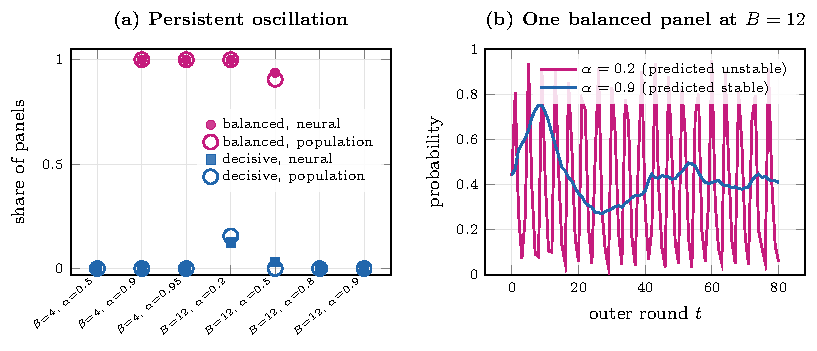
\includegraphics[width=0.98\textwidth]{exp_cycles.pdf}
\caption{Planted cycles. \textbf{(a)} Share of panels whose answer probabilities still oscillate over the last 30 of 80 rounds, neural (filled) against the noise-free population recursion from the same initial scores (open), for balanced (majority cycle) and decisive (Condorcet winner) panels. \textbf{(b)} One balanced panel at the fixed target $B=12$: the probability of one answer under $\alpha=0.2$, predicted unstable, and $\alpha=0.9$, predicted stable.}
\label{fig:exp-cycles}
\end{figure}
